\documentclass[conference]{IEEEtran}
\IEEEoverridecommandlockouts

\usepackage{cite}
\usepackage{amsmath,amssymb,amsfonts}
\usepackage{graphicx}
\usepackage{textcomp}
\usepackage{xcolor}
\usepackage{booktabs}
\usepackage{url}
\usepackage{tikz}
\usetikzlibrary{positioning,arrows.meta}
\usepackage{algorithm}
\usepackage{algpseudocode}
\renewcommand{\ttdefault}{cmtt}
\setlength{\abovedisplayskip}{4pt plus 2pt minus 2pt}
\setlength{\belowdisplayskip}{4pt plus 2pt minus 2pt}
\setlength{\abovedisplayshortskip}{2pt plus 2pt minus 2pt}
\setlength{\belowdisplayshortskip}{2pt plus 2pt minus 2pt}
\setlength{\textfloatsep}{6pt plus 2pt minus 2pt}
\setlength{\intextsep}{6pt plus 2pt minus 2pt}
\setlength{\floatsep}{4pt plus 2pt minus 2pt}

\begin{document}

\title{Master Comparator: Training-Free Few-Shot Gallery Matching for Counterfeit Product Authentication}

\author{
\IEEEauthorblockN{1\textsuperscript{st} Malapati Sahasra}
\IEEEauthorblockA{
\textit{Dept. of AI and Emerging Technology} \\
\textit{Chinmaya Vishwavidyapeeth} \\
Ernakulam, Kerala, India \\
malapati.cvv241195@cvv.ac.in}
\and
\IEEEauthorblockN{2\textsuperscript{nd} Kothuri Rushya Sai}
\IEEEauthorblockA{
\textit{Dept. of AI and Emerging Technology} \\
\textit{Chinmaya Vishwavidyapeeth} \\
Ernakulam, Kerala, India \\
kothuri.cvv241242@cvv.ac.in}
\and
\IEEEauthorblockN{3\textsuperscript{rd} B. R. Sneha}
\IEEEauthorblockA{
\textit{Dept. of AI and Emerging Technology} \\
\textit{Chinmaya Vishwavidyapeeth} \\
Ernakulam, Kerala, India \\
belodu.cvv241233@cvv.ac.in}
\and
\IEEEauthorblockN{4\textsuperscript{th} Dr. Uma Narayanan}
\IEEEauthorblockA{
\textit{Dept. of AI and Emerging Technologies} \\
\textit{Chinmaya Vishwavidyapeeth} \\
Ernakulam, Kerala, India \\
uma.narayanan@cvv.ac.in}
}

\maketitle

\begin{abstract}
Buyers on e-commerce marketplaces must judge product authenticity from a
few listing photographs. We present \emph{Master Comparator}, a
training-free, one-class \emph{few-shot} verifier: a test photograph is
compared against a small support gallery of $k$ genuine reference images
(no counterfeit examples and no learned parameters) by three interpretable
checks --- ORB keypoint matching, hue--saturation histogram correlation,
and OCR brand-text verification --- with an optional barcode check,
combined by an ``allow one miss'' vote. On 1{,}600 photographs of five
brands (Nike, Puma, Adidas, Gucci, Louis Vuitton; 93.6\% unmodified real
photographs) with a strictly held-out gallery of $k{=}20$ images (about four
per brand), the cascade reaches 58.06\% accuracy, 70.48\% precision and
27.75\% recall (58.5$\pm$1.3\% accuracy over 20 random galleries), at a
mean CPU latency of 155~ms per image. We additionally report: performance
as a function of $k$ (cascade F1 rises from 0.03 at $k{=}1$ to 0.58 at
$k{=}68$); comparisons against SIFT, perceptual-hash, HOG and pretrained
CNN-embedding baselines on the same gallery, plus a supervised upper
reference; robustness under eight capture conditions; and a failure
analysis showing that the color check's discriminative power stems
largely from background and photography style rather than product
color. These results define where a training-free few-shot verifier is
and is not suitable for deployment.
\end{abstract}

\begin{IEEEkeywords}
counterfeit detection, few-shot verification, training-free, gallery
matching, ORB, HSV histogram, OCR, e-commerce, robustness, shortcut learning
\end{IEEEkeywords}

\section{Introduction}
\label{sec:intro}

Counterfeit goods are routinely sold alongside genuine ones on e-commerce
marketplaces, and buyers must judge authenticity from a few listing
photographs. Subtle indicators --- a wrong shade, altered logo
proportions, a misspelled brand name --- are easy to miss by eye.

Most recent work trains deep classifiers on large, brand-specific corpora
\cite{footwear2024,fakelogo2024}. These require labeled counterfeit
examples, GPU training and retraining for every new product line. Many
practical settings --- a small seller, a new product launch, an edge
device --- have neither counterfeit training data nor a GPU, but
\emph{can} supply a handful of photographs of the genuine product.

This paper studies that setting: \emph{one-class, few-shot verification
without training}. Given only $k$ genuine reference photographs, can
interpretable matching decide whether a new photograph shows a genuine
item? Our contributions are:

\begin{enumerate}
    \item \textbf{A training-free few-shot formulation} (Master Comparator)
    in which logo and color checks score a test image by its best match
    over a support gallery of $k$ genuine images (Sec.~\ref{sec:problem}),
    with a fully specified, leakage-free evaluation protocol
    (Sec.~\ref{sec:protocol}).
    \item \textbf{A documented five-brand evaluation set} of 1{,}600 real
    photographs with a held-out gallery, per-image provenance, and an
    audit for gallery leakage and duplicated images (Sec.~\ref{sec:dataset}).
    \item \textbf{An extensive empirical study}: a gallery-size ($k$-shot)
    sweep with 20 random galleries per size, six baselines plus a
    supervised reference, robustness under eight capture conditions, and a
    failure analysis that exposes a background shortcut in the color cue
    (Sec.~\ref{sec:results}).
\end{enumerate}

Code, evaluation scripts and an interactive demonstration are
public.\footnote{Code: \url{https://github.com/MalapatiSahasra/fake-product-detection}. Demo: \url{https://web-tau-indol-42.vercel.app}}

\section{Related Work}
\label{sec:related}

\textbf{Counterfeit and logo detection.} A CNN trained on 3{,}000 genuine
and 2{,}000 counterfeit sneaker photographs reported over 95\% accuracy,
outperforming an SVM~\cite{footwear2024}; the Roboflow ``Original or Fake
Shoes'' dataset provides bounding-box labels for Nike models
\cite{roboflow2024}; fake-logo detectors report over 99\% accuracy on
curated imagery~\cite{fakelogo2024}. All are supervised and need labeled
counterfeits.

\textbf{Few-shot recognition.} Matching networks~\cite{vinyals2016} and
prototypical networks~\cite{snell2017} classify a query by comparing it
with a small labeled support set, but learn the embedding by episodic
meta-training. Our system shares the support-set protocol but learns
nothing: comparisons use fixed classical descriptors
\cite{orb2011,lowe2004,opencv} and need only the genuine class.

\textbf{Shortcut learning.} Classifiers can succeed by exploiting
spurious dataset cues such as backgrounds~\cite{geirhos2020}. We test for
this explicitly (Sec.~\ref{sec:failures}).

\begin{table}[t]
\caption{Positioning Against Related Work}
\label{tab:related}
\centering
\resizebox{\columnwidth}{!}{%
\begin{tabular}{lcccc}
\toprule
System & Training & Counterfeit labels & Brands & GPU \\
\midrule
Footwear CNN/SVM~\cite{footwear2024} & Yes & Yes & 1 & Yes \\
Fake-logo detector~\cite{fakelogo2024} & Yes & Yes & Multi (curated) & Yes \\
Roboflow detector~\cite{roboflow2024} & Yes & Yes & 1 & Yes \\
Proto./matching nets~\cite{snell2017,vinyals2016} & Meta-train & Per episode & -- & Yes \\
\textbf{This work} & \textbf{None} & \textbf{No} & \textbf{5, uncurated} & \textbf{No} \\
\bottomrule
\end{tabular}}
\end{table}

Table~\ref{tab:related} summarizes the trade-off: supervised systems
report higher accuracy on narrower, curated domains, whereas this work
targets zero training cost, no counterfeit labels and CPU-only inference
on a heterogeneous pool. Sec.~\ref{sec:baselines} quantifies the gap to a
supervised reference on the same data.

\section{Problem Formulation and System}
\label{sec:problem}

\subsection{Why Few-Shot, Not Zero-Shot}

Let $G = \{g_1,\dots,g_k\}$ be a \emph{support gallery} of $k$
photographs known to be genuine. Given a test photograph $t$, the task is
to decide \textsc{Authentic} or \textsc{Counterfeit}. The setting is
\emph{few-shot} because the decision depends on $k$ labeled exemplars of
the genuine class (here $k{=}20$ across five brands, i.e.\ about four per
brand); it is not zero-shot, which would require recognizing genuineness
with no exemplars at all. It is \emph{one-class} because no counterfeit
exemplars are used, and \emph{training-free} because no parameter is
fitted to data: the gallery is only compared against. Only the OCR check
is exemplar-free, as it uses brand strings alone.

\subsection{Gallery Matching and Cascade}

\begin{figure}[t]
\centering
\resizebox{\columnwidth}{!}{%
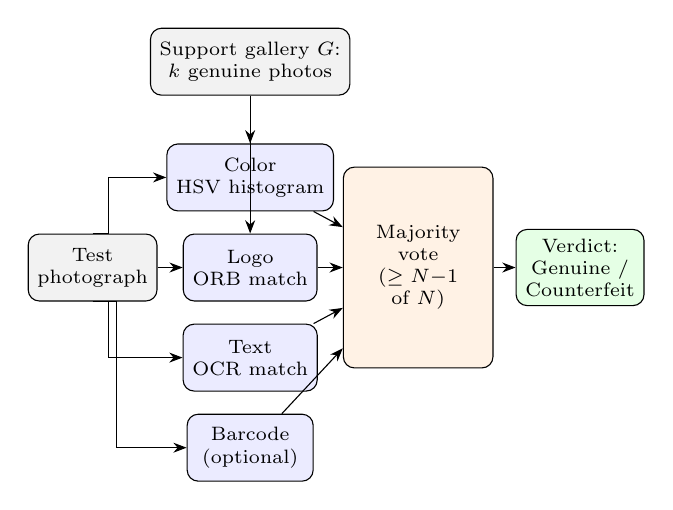
\begin{tikzpicture}[
  box/.style={draw, rounded corners, minimum width=1.6cm, minimum height=0.85cm, align=center, font=\scriptsize},
  node distance=0.28cm and 0.32cm
]
\node[box, fill=gray!10] (input) {Test\\photograph};
\node[box, right=0.32cm of input, fill=blue!8] (logo) {Logo\\ORB match};
\node[box, above=of logo, fill=blue!8] (color) {Color\\HSV histogram};
\node[box, below=of logo, fill=blue!8] (typo) {Text\\OCR match};
\node[box, below=of typo, fill=blue!8] (qr) {Barcode\\(optional)};
\node[box, right=0.32cm of logo, minimum width=1.9cm, minimum height=2.55cm, fill=orange!10] (vote) {Majority\\vote\\($\geq N{-}1$\\of $N$)};
\node[box, right=0.28cm of vote, fill=green!10] (out) {Verdict:\\Genuine /\\Counterfeit};
\node[box, above=1.75cm of logo, fill=gray!10, minimum height=0.85cm] (gallery) {Support gallery $G$:\\$k$ genuine photos};

\draw[-Stealth] (input) -- (logo);
\draw[-Stealth] (input.north) -- ++(0.2,0) |- (color.west);
\draw[-Stealth] (input.south) -- ++(0.2,0) |- (typo.west);
\draw[-Stealth] (input.south) -- ++(0.3,0) |- (qr.west);
\draw[-Stealth] (gallery.south) -- (color.north);
\draw[-Stealth] (gallery) -- (logo);
\draw[-Stealth] (logo) -- (vote);
\draw[-Stealth] (color) -- (vote);
\draw[-Stealth] (typo) -- (vote);
\draw[-Stealth] (qr) -- (vote);
\draw[-Stealth] (vote) -- (out);
\end{tikzpicture}%
}
\caption{Master Comparator. Logo and color checks take the best match over the support gallery $G$; text and barcode checks are gallery-independent. A photograph is accepted if at most one active module disagrees.}
\label{fig:architecture}
\end{figure}

Fig.~\ref{fig:architecture} shows the system. The logo and color modules
score $t$ by its best match in the gallery:
\begin{equation}
s_{\text{module}}(t) = \max_{g_i \in G} \; \text{score}(t, g_i)
\label{eq:gallery}
\end{equation}
Each module $m$ thresholds its score into a pass/fail decision. With $N$
active modules ($N{=}4$ when a barcode is expected, otherwise $N{=}3$),
\begin{equation}
\text{score}(t) = \sum_{m=1}^{N} \mathbb{1}\left[\text{module}_m(t) = \text{pass}\right]
\end{equation}
and $t$ is \textsc{Authentic} iff $\text{score}(t) \geq N-1$. All modules
always run (Algorithm~\ref{alg:cascade}), so every verdict is explainable
by its per-module scores.

\begin{algorithm}[t]
\caption{Master Comparator Verification}
\label{alg:cascade}
\begin{algorithmic}[1]
\Require test image $t$, genuine gallery $G$, brand strings $B$, barcode expectation $q$ (optional)
\Ensure verdict $\in \{\textsc{Authentic}, \textsc{Counterfeit}\}$
\State $r_{\text{logo}} \gets$ \Call{LogoMatch}{$t$, $G$}; $r_{\text{color}} \gets$ \Call{ColorMatch}{$t$, $G$}
\State $r_{\text{text}} \gets$ \Call{TextMatch}{$t$, $B$}
\If{barcode check applicable to data source}
    \State $r_{\text{code}} \gets$ \Call{BarcodeCheck}{$t$, $q$}; $N \gets 4$
\Else
    \State $N \gets 3$
\EndIf
\State $\text{score} \gets \sum \mathbb{1}[r_m = \text{pass}]$ over active modules
\State \Return \textsc{Authentic} \textbf{if} $\text{score} \geq N - 1$ \textbf{else} \textsc{Counterfeit}
\end{algorithmic}
\end{algorithm}

\subsection{Verification Modules}
\label{sec:modules}

\textbf{Logo (ORB).} Up to 1{,}000 ORB keypoints~\cite{orb2011} are
detected per image; descriptors are matched by brute force under Hamming
distance with $k$-NN ($k{=}2$), keeping a match only if it passes Lowe's
ratio test~\cite{lowe2004}, $d(m) < 0.75\, d(n)$. The module passes if the
best gallery image yields at least $\tau_{\text{logo}}{=}15$ good matches.

\textbf{Color (HS histogram).} Images are converted to HSV and a
$50\times60$ Hue--Saturation histogram is computed (Value excluded for
exposure invariance), min--max normalized, and compared by Pearson
correlation; the module passes if the best gallery correlation is at
least $\tau_{\text{color}}{=}0.70$.

\textbf{Text (OCR).} A bilateral filter and global Otsu threshold precede
Tesseract~\cite{tesseract2007} in sparse-text mode (PSM~11). The cleaned
text is compared with the brand strings \{\textsc{Nike}, \textsc{Puma},
\textsc{Adidas}, \textsc{Gucci}, \textsc{LV}\} by a sliding-window
Ratcliff/Obershelp ratio $2M/T$~\cite{ratcliff1988}; the module passes at
$\tau_{\text{text}}{=}0.80$, which tolerates OCR noise but rejects
misspellings such as ``NUMA'' for ``PUMA''.

\textbf{Barcode (optional).} QR/EAN-13/Code-128 symbols are decoded with
ZBar~\cite{zbar} and checked against an expected serial pattern. Only 1 of
the 1{,}565 raw source photographs contains a decodable code, so this
module is excluded ($N{=}3$) in all experiments; it remains available for
authentication-tag photographs.

\textbf{Complexity.} For a gallery of size $k$, logo matching costs
$O(k\, n^2)$ for $n$ keypoints and color matching $O(k\, b)$ for
$b{=}3{,}000$ bins; OCR is independent of $k$. Table~\ref{tab:timing}
reports measured latency.

\begin{table}[t]
\caption{Single-Thread Latency per Image ($k{=}20$, 60 Images)}
\label{tab:timing}
\centering
\begin{tabular}{lrl}
\toprule
Stage & Mean (ms) & Scales with $k$? \\
\midrule
Decode + resize     & 3.2 & No \\
Logo (ORB extract + match) & 64.3 & Yes, $O(k)$ \\
Color (HS histogram)   & 1.0 & Yes, $O(k)$ \\
Text (OCR)          & 86.1 & No \\
\midrule
\textbf{Total} & \textbf{154.5} & median 136.9, p95 275.1 \\
\bottomrule
\end{tabular}
\end{table}

\section{Dataset}
\label{sec:dataset}

\subsection{Source and Composition}

Photographs come from the Kaggle ``Fake Brand Dataset (Adidas, Nike,
Gucci, Puma, LV)'' (CC BY-NC 4.0)~\cite{kaggledata}, whose publisher
assigns each image a genuine/counterfeit label. The images are uncurated
marketplace-style photographs: studio product shots on white backgrounds,
handheld photographs, worn-on-foot and lifestyle images. All five brand
subsets were used: 855 genuine and 710 counterfeit raw images (1{,}565).
Table~\ref{tab:dataset-brand} gives the per-brand split at each stage.

\begin{table}[t]
\caption{Images per Brand: Raw Source, Held-Out Gallery, Evaluation Set (Genuine/Counterfeit)}
\label{tab:dataset-brand}
\centering
\begin{tabular}{lccc}
\toprule
Brand & Raw (G/C) & Gallery (G) & Evaluation (G/C) \\
\midrule
Nike   & 260 / 253 & 21 & 240 / 278 \\
Puma   & 199 / 91  & 16 & 188 / 106 \\
Adidas & 178 / 140 & 14 & 168 / 160 \\
Gucci  & 190 / 152 & 15 & 178 / 175 \\
LV     & 28 / 74   & 2  & 26 / 81 \\
\midrule
\textbf{Total} & \textbf{855 / 710} & \textbf{68} & \textbf{800 / 800} \\
\bottomrule
\end{tabular}
\end{table}

\subsection{Held-Out Gallery and Augmentation}

A seeded 8\% of genuine images per brand (68 images) was reserved as the
gallery pool and excluded from evaluation, so no test image can match
itself. The remaining 787 genuine and 710 counterfeit images were topped
up to exactly 800 per class by deterministic augmentation (seed 42) of a
random sample of seeds: rotation in $[-15^\circ,15^\circ]$, brightness
scaling of the V channel in $[0.6,1.4]$, and Gaussian noise
$\sigma\in[5,20]$. A per-image manifest records the source seed and the
exact parameters, so the set is regenerable byte-for-byte.

\subsection{Exact Dataset Statistics}

\begin{table}[t]
\caption{Exact Evaluation-Set Statistics (from the Per-Image Manifests)}
\label{tab:stats}
\centering
\resizebox{\columnwidth}{!}{%
\begin{tabular}{lrrr}
\toprule
Statistic & Genuine & Counterfeit & Total \\
\midrule
Samples in evaluation set & 800 & 800 & 1{,}600 \\
\quad Unmodified photographs & 787 & 710 & 1{,}497 \\
\quad Augmented images & 13 & 90 & 103 \\
Genuine : counterfeit ratio & \multicolumn{3}{c}{1 : 1 (800 : 800)} \\
Held-out gallery pool (not evaluated) & 68 & -- & 68 \\
\midrule
\multicolumn{4}{l}{\textit{Images per category (brand), evaluation set}} \\
\quad Nike / Puma / Adidas & 240 / 188 / 168 & 278 / 106 / 160 & 518 / 294 / 328 \\
\quad Gucci / LV & 178 / 26 & 175 / 81 & 353 / 107 \\
\midrule
\multicolumn{4}{l}{\textit{Illumination condition (augmented images, brightness factor $b$)}} \\
\quad Low light ($b < 0.85$) & 4 & 19 & 23 \\
\quad Normal ($0.85 \leq b \leq 1.15$) & 7 & 44 & 51 \\
\quad Bright ($b > 1.15$) & 2 & 27 & 29 \\
\quad Original capture (no label) & 787 & 710 & 1{,}497 \\
\midrule
\multicolumn{4}{l}{\textit{Origin of images}} \\
\quad Distinct source photographs & 787 & 710 & 1{,}497 \\
\quad Source photos with 2 outputs & 13 & 90 & 103 \\
\quad Max.\ outputs per source photo & 2 & 2 & -- \\
\bottomrule
\end{tabular}}
\end{table}

Table~\ref{tab:stats} lists the exact counts, all computed from the
per-image manifests. Illumination labels apply only to the 103 augmented
images, bucketed by their recorded brightness factor (two decimals); the
1{,}497 unmodified photographs keep their original lighting. By
construction, \emph{multiple images originate from the same photograph}
only through augmentation: each augmented image is derived from exactly
one recorded source photograph, and 103 source photographs (13 genuine, 90
counterfeit) contribute two images each (original plus one augmented
copy). Whether two \emph{different} source photographs show the same
physical item is not recorded by the dataset publisher. We therefore
measured it with the near-duplicate audit below: 65 evaluation images
(4.1\%, in 49 same-label pairs) have a near-identical photograph under a
different source file and very likely show the same item. Photographs of
one item from clearly different angles cannot be detected by this audit,
so this figure is a lower bound.

\subsection{Leakage and Duplicate Audit}
\label{sec:dupaudit}

Because the source is uncurated, we searched for near-duplicates (pHash
Hamming distance $\leq 4$ and MobileNetV2 embedding cosine $\geq 0.95$)
across all 1{,}668 images. Three genuine test images have a near-duplicate
in the 68-image gallery pool (one in the 20-image gallery used below).
Eight image pairs appear under \emph{both} labels (16 images; five pairs
have identical perceptual hashes), i.e.\ label noise in the source. A
further 49 same-label pairs come from different seed photographs.
Removing the 19 leaked or cross-labeled images changes the main result
negligibly (F1 0.398 $\rightarrow$ 0.400), so they are retained to keep
the set regenerable, and the issue is reported here.

\section{Evaluation Protocol}
\label{sec:protocol}

\begin{table}[t]
\caption{Fixed Settings Used in All Experiments}
\label{tab:settings}
\centering
\setlength{\tabcolsep}{4pt}
\begin{tabular}{ll}
\toprule
Setting & Value \\
\midrule
Pre-processing & long side $\leq$1{,}600 px (area interpolation) \\
ORB / ratio / $\tau_{\text{logo}}$ & 1{,}000 keypoints / 0.75 / 15 matches \\
HS bins / $\tau_{\text{color}}$ & $50\times60$ / 0.70 correlation \\
OCR / $\tau_{\text{text}}$ & Tesseract 4.1.1, PSM 11, Otsu / 0.80 \\
Vote & $\geq N{-}1$ of $N{=}3$ (barcode excluded) \\
Main gallery & $k{=}20$ sampled from 68 (seed 42) \\
Variance study & 20 random galleries per $k$ (seeds 1000--1019) \\
Software & Python 3.10, OpenCV 5.0, scikit-learn 1.7 \\
Hardware & 4-vCPU Linux VM, Apple-silicon laptop, no GPU \\
\bottomrule
\end{tabular}
\end{table}

The protocol is as follows (settings in Table~\ref{tab:settings}):
\begin{enumerate}
\item \textbf{Split.} Gallery pool (68 genuine) and evaluation set (800
genuine, 800 counterfeit) are disjoint by construction
(Sec.~\ref{sec:dataset}).
\item \textbf{Thresholds.} The module thresholds and vote rule are fixed a
priori and are \emph{not} tuned on the evaluation set; every image is
scored once.
\item \textbf{Metrics.} \textsc{Genuine} is the positive class. We report
accuracy, precision, recall, F1, false-acceptance rate
FAR $=FP/(FP+TN)$, and threshold-free ROC-AUC of continuous scores.
\item \textbf{Gallery variance.} Because results depend on which $k$
images form $G$, each $k\in\{1,2,5,10,20,40,68\}$ is evaluated on 20
random galleries and reported as mean $\pm$ standard deviation.
\item \textbf{Baselines.} Every baseline uses the same gallery and the
same best-match rule (Eq.~\ref{eq:gallery}). Because baselines have no
published thresholds, each continuous score (including our modules') is
thresholded by 5-fold cross-validation: the threshold maximizing accuracy
on four folds is applied to the fifth. Folds are grouped by source
photograph so augmented copies never span folds.
\item \textbf{Robustness.} A seeded, class-balanced subset of 400
unaugmented images (200/200) is re-scored under eight perturbations
applied to the test image only (the gallery is unchanged).
\item \textbf{Latency.} Single-thread wall-clock time over 60 images
including decoding (Table~\ref{tab:timing}).
\end{enumerate}

\section{Experimental Results}
\label{sec:results}

\subsection{Main Result}

\begin{table}[t]
\caption{Main Result ($k{=}20$, 1{,}600 Images, $\geq$2 of 3 Vote)}
\label{tab:metrics}
\centering
\begin{tabular}{lrr|lr}
\toprule
 & Pred.\ Gen. & Pred.\ Cf. & Metric & Value \\
\midrule
Genuine     & TP = 222 & FN = 578 & Accuracy  & 58.06\% \\
Counterfeit & FP = 93  & TN = 707 & Precision & 70.48\% \\
 & & & Recall & 27.75\% \\
 & & & F1 / FAR & 0.398 / 11.6\% \\
\midrule
\multicolumn{3}{l}{20 random galleries ($k{=}20$)} & Accuracy & 58.5 $\pm$ 1.3\% \\
 & & & F1 & 0.390 $\pm$ 0.046 \\
\bottomrule
\end{tabular}
\end{table}

Table~\ref{tab:metrics} reports the cascade on the full evaluation set.
The verifier is conservative: 70.5\% of accepted photographs are genuine
and 11.6\% of counterfeits are accepted, but only 27.8\% of genuine
photographs are recognized. Over 20 random galleries the figures vary by
about $\pm$1.3 points of accuracy, so the qualitative profile does not
depend on the particular gallery drawn.

\subsection{Per-Brand Results}
\label{sec:perbrand}

\begin{table}[t]
\caption{Cascade Results by Brand ($k{=}20$, seed 42)}
\label{tab:perbrand}
\centering
\begin{tabular}{lrrrrr}
\toprule
Brand & $n$ & Gallery & Acc. & Prec. & Recall \\
\midrule
Adidas & 328 & 7 & 63.4\% & 82.4\% & 36.3\% \\
Gucci  & 353 & 3 & 54.1\% & 64.3\% & 20.2\% \\
LV     & 107 & 0 & 69.2\% & 26.7\% & 15.4\% \\
Nike   & 518 & 6 & 60.4\% & 68.8\% & 26.7\% \\
Puma   & 294 & 4 & 48.6\% & 74.0\% & 30.3\% \\
\bottomrule
\end{tabular}
\end{table}

Table~\ref{tab:perbrand} also lists how many of the 20 gallery images
belong to each brand. Adidas, with the most references (7), has the
highest recall and precision; LV has none in this draw and the lowest
precision (26.7\%, from 26 genuine against 81 counterfeit images). LV's
high accuracy simply reflects its 76\% counterfeit share. Brand-stratified
gallery sampling is therefore recommended in practice.

\subsection{Module Ablation}
\label{sec:ablation}

\begin{table}[t]
\caption{Standalone Modules vs.\ Vote Rules ($k{=}20$)}
\label{tab:ablation}
\centering
\begin{tabular}{lrrrr}
\toprule
Configuration & Acc. & Prec. & Recall & F1 \\
\midrule
Logo alone          & 52.3\% & 52.8\% & 44.4\% & 0.482 \\
Color alone        & 66.9\% & 69.1\% & 61.4\% & 0.650 \\
Text alone          & 49.9\% & 45.5\% &  1.3\% & 0.024 \\
Cascade, $\geq 1$ of 3 & 60.9\% & 58.0\% & 79.0\% & \textbf{0.669} \\
Cascade, $\geq 2$ of 3 & 58.1\% & 70.5\% & 27.8\% & 0.398 \\
Cascade, $\geq 3$ of 3 & 50.1\% & 100.0\% & 0.3\% & 0.005 \\
\bottomrule
\end{tabular}
\end{table}

Table~\ref{tab:ablation} shows that color alone (F1 0.650) outperforms
the $\geq$2-of-3 cascade (0.398). OCR read some text in 66\% of images,
but only 22 of 1{,}600 contained a legible brand string (10 genuine, 12
counterfeit), so text recall is 1.3\% and requiring it to agree discards
most of color's correct acceptances. The vote threshold is thus a
deployment parameter that trades precision for recall.

\subsection{Effect of Gallery Size ($k$-Shot)}
\label{sec:kshot}

\begin{figure}[t]
\centering
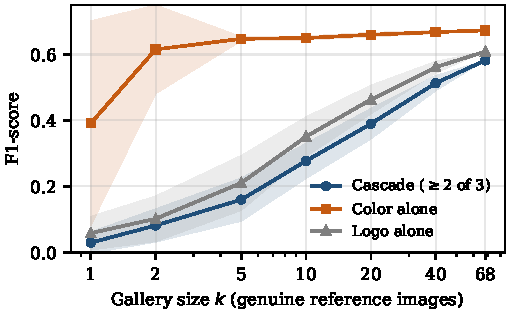
\includegraphics[width=\columnwidth]{fig_kshot.pdf}
\caption{F1 versus gallery size $k$ (mean $\pm$ s.d.\ over 20 random galleries; $k{=}68$ uses the whole pool).}
\label{fig:kshot}
\end{figure}

Fig.~\ref{fig:kshot} shows the few-shot behavior. Cascade F1 grows
monotonically from 0.03 ($k{=}1$) through 0.28 ($k{=}10$) and 0.39
($k{=}20$) to 0.58 ($k{=}68$), at which point accuracy is 64.3\% and
recall 49.7\%. Precision decreases slightly with $k$ (73.4\% at
$k{=}20$ to 70.2\% at $k{=}68$), because a larger gallery also offers
counterfeits more chances to match. The color module saturates near
F1 0.65 by $k{=}5$, while logo matching keeps improving, which shows that
recall is limited mainly by gallery coverage.

\subsection{Baseline Comparison}
\label{sec:baselines}

\begin{table}[t]
\caption{Baselines on the Same Gallery (Cross-Validated Threshold)}
\label{tab:baselines}
\centering
\setlength{\tabcolsep}{3pt}
\begin{tabular}{lcccc}
\toprule
Method (best match over $G$) & \multicolumn{3}{c}{$k{=}20$} & $k{=}68$ \\
 & AUC & Acc. & F1 & AUC \\
\midrule
\multicolumn{5}{l}{\textit{Training-free, classical}} \\
ORB matching (ours, logo)  & 0.517 & 53.0\% & 0.382 & 0.551 \\
HS color (ours)          & 0.705 & 68.8\% & 0.615 & 0.724 \\
OCR text (ours)           & 0.389 & 50.0\% & 0.292 & 0.389 \\
SIFT matching~\cite{lowe2004} & 0.564 & 53.8\% & 0.549 & 0.573 \\
Perceptual hash (pHash)~\cite{zauner2010} & 0.689 & 62.9\% & 0.582 & 0.728 \\
HOG cosine~\cite{dalal2005} & 0.346 & 51.0\% & 0.137 & 0.443 \\
\midrule
\multicolumn{5}{l}{\textit{Pretrained deep features, no fine-tuning}} \\
MobileNetV2 embedding~\cite{sandler2018} & 0.716 & 65.8\% & 0.624 & 0.767 \\
\midrule
\multicolumn{5}{l}{\textit{Uses counterfeit labels (reference only)}} \\
Weighted fusion of our 3 scores (LR) & 0.708 & 66.8\% & 0.661 & 0.721 \\
Supervised LR on MobileNetV2 & 0.854 & 78.8\% & 0.790 & -- \\
\midrule
Master Comparator, fixed $\geq$2 of 3 & -- & 58.1\% & 0.398 & -- \\
Master Comparator, fixed $\geq$1 of 3 & -- & 60.9\% & 0.669 & -- \\
\bottomrule
\end{tabular}
\end{table}

Table~\ref{tab:baselines} compares six training-free matchers under the
same gallery and best-match rule. Among classical methods, our HS color
score achieves the highest AUC (0.705), ahead of perceptual hashing
(0.689) and SIFT (0.564). An ImageNet-pretrained MobileNetV2 embedding
without fine-tuning is slightly stronger (0.716 at $k{=}20$, 0.767 at
$k{=}68$) but needs a deep model and no longer gives a per-module
explanation. Learning only four weights to fuse our three scores raises
F1 to 0.661 without tuning anything else. A supervised logistic-regression
probe on MobileNetV2 features, which needs labeled counterfeits, reaches
0.854 AUC and 78.8\% accuracy; this marks the price of the training-free,
one-class setting on this dataset. Notably, ORB and SIFT keypoint
matching are near chance (AUC 0.52--0.57) across brands, as expected for
a gallery spanning many different products.

\subsection{Robustness under Practical Capture Conditions}
\label{sec:robust}

\begin{table}[t]
\caption{Robustness ($n{=}400$ Unaugmented Images, $k{=}20$; Perturbation on Test Image Only)}
\label{tab:robust}
\centering
\setlength{\tabcolsep}{3pt}
\begin{tabular}{lrrrrrr}
\toprule
Condition & Acc. & Prec. & Rec. & FAR & \multicolumn{2}{c}{AUC} \\
 & & & & & Color & CNN \\
\midrule
Clean                          & 56.8 & 68.5 & 25.0 & 11.5 & 0.724 & 0.679 \\
Blur ($\sigma{=}3$)            & 64.7 & 72.5 & 47.5 & 18.0 & 0.720 & 0.665 \\
JPEG ($q{=}20$)                & 53.5 & 56.6 & 30.0 & 23.0 & 0.718 & 0.680 \\
Low-res ($\tfrac14$ size)      & 60.0 & 64.9 & 43.5 & 23.5 & 0.721 & 0.663 \\
Rotation ($30^\circ$)          & 59.3 & 70.3 & 32.0 & 13.5 & 0.722 & 0.707 \\
Perspective (15\%)             & 60.8 & 75.3 & 32.0 & 10.5 & 0.730 & 0.708 \\
Occlusion (25\% area)          & 48.2 & 47.7 & 36.5 & \textbf{40.0} & 0.699 & 0.562 \\
Low light ($\times0.45$+noise) & 50.2 & (1/1) & 0.5 & 0.0 & \textbf{0.339} & 0.653 \\
Warm color cast               & 50.2 & 60.0 & 1.5 & 1.0 & \textbf{0.219} & 0.694 \\
\bottomrule
\end{tabular}
\end{table}

Table~\ref{tab:robust} tests eight conditions typical of buyer- or
seller-captured photographs. Geometric changes (rotation, perspective)
are tolerated. Blur, heavy JPEG compression and low resolution
\emph{raise} recall but also raise the false-acceptance rate (to
18--24\%), because smoothing produces generic keypoints that match more
gallery images. A 25\%-area occlusion is the most harmful case for
security, accepting 40\% of counterfeits. Low light and a warm color
cast make the color module fail completely: its AUC falls \emph{below}
chance (0.34 and 0.22) and the cascade rejects almost everything, whereas
the CNN embedding stays near 0.65--0.69. Photometric normalization
(gray-world white balance with chromatic masking) did not recover the
color cue (AUC 0.46 under low light, 0.41 under color cast). The system
should therefore be deployed only with controlled capture
(consistent lighting and white balance, unobstructed view).

\subsection{Failure-Case Analysis}
\label{sec:failures}

\begin{figure*}[t]
\centering
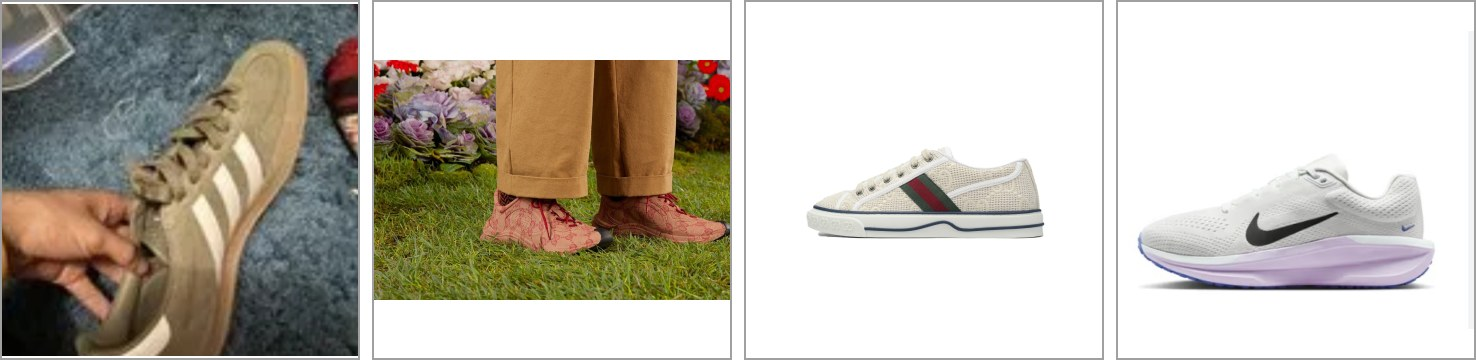
\includegraphics[width=0.92\textwidth]{fig_failures.jpg}
\caption{Representative errors ($k{=}20$). (a) Genuine Adidas, handheld on carpet: best color correlation 0.18, 16 ORB matches $\rightarrow$ rejected. (b) Genuine Gucci, worn outdoors: color 0.19, 10 matches $\rightarrow$ rejected. (c) Counterfeit Gucci and (d) counterfeit Nike studio shots on white: color 1.00/1.00, 15/17 matches $\rightarrow$ accepted.}
\label{fig:failures}
\end{figure*}

\begin{table}[t]
\caption{Error Analysis by Near-White Background Fraction}
\label{tab:failbg}
\centering
\begin{tabular}{lrrrr}
\toprule
Background fraction & $n$ & Genuine & Recall & FAR \\
\midrule
$<$0.10      & 426 & 130 & 6.9\%  & 4.4\% \\
0.10--0.30   & 392 & 124 & 5.6\%  & 8.2\% \\
0.30--0.60   & 254 & 103 & 31.1\% & 19.9\% \\
$\geq$0.60   & 528 & 443 & 39.3\% & 32.9\% \\
\bottomrule
\end{tabular}
\end{table}

Fig.~\ref{fig:failures} shows typical errors, and they follow a clear
pattern. Genuine photographs taken by hand or in lifestyle settings are
rejected, while counterfeit studio shots on white backgrounds are
accepted. To quantify this we measured each image's fraction of
near-white pixels (S$<$30, V$>$200). Genuine evaluation images average
52\% background against 24\% for counterfeits, and the gallery averages
50\%. Background fraction \emph{alone} separates the classes with AUC
0.747, higher than the color module (0.705). When the color histogram
is restricted to chromatic product pixels (S$\geq$40, V$\geq$40), its AUC
drops to 0.466, i.e.\ chance. The color module's apparent
discriminative power therefore comes mainly from \emph{photography
style}, a dataset shortcut~\cite{geirhos2020}, rather than from product
color. Table~\ref{tab:failbg} confirms this: recall is 39.3\% on
white-background images but under 7\% on others, and false acceptances
concentrate on white-background counterfeits (FAR 32.9\%).

Module-level patterns support this reading. Of the 578 false negatives,
272 passed only color (failed logo), 136 passed only logo, and 168 failed
all modules. Of the 93 false positives, 86 passed both logo and color,
i.e.\ counterfeit studio shots that resemble the studio-style gallery.
Some cross-labeled duplicates (Sec.~\ref{sec:dupaudit}) are also
counted as errors although they are visually indistinguishable.

\section{Discussion}
\label{sec:discussion}

\textbf{What the results support.} With about four genuine references per
brand and no training, the verifier is conservative (precision 70.5\%,
FAR 11.6\%) and fully explainable at 155~ms per image on a CPU. Recall
rises steadily with gallery size (Fig.~\ref{fig:kshot}), and the vote
threshold or a small learned weighting moves the operating point
(Tables~\ref{tab:ablation},~\ref{tab:baselines}).

\textbf{What they do not support.} The results do not support
unsupervised brand-level authentication of arbitrary marketplace photos.
On this dataset the color cue largely detects photography style, keypoint
matching across different products is near chance, and occlusion or
lighting changes either raise false acceptance (40\% under occlusion) or
disable the color check. We therefore scope the deployment claim: Master
Comparator is suited to \emph{controlled-capture, per-SKU verification}
--- for example a checkpoint or seller-onboarding flow in which the item
is photographed against a fixed background under fixed lighting and
compared with references of the same SKU --- and as a first-stage triage
that routes uncertain listings to human review. It should not be used as
the sole authority on unconstrained marketplace images.

\textbf{Barcode.} 1{,}564 of 1{,}565 raw photographs carry no readable
code, so barcode verification needs deliberately captured authentication
tags.

\subsection{Threats to Validity}
\label{sec:threats}

\textbf{Labels and duplicates.} Labels come from the dataset publisher;
eight cross-labeled duplicate pairs show they are imperfect
(Sec.~\ref{sec:dupaudit}). \textbf{Independence.} Whether different raw
photographs depict the same physical unit is undocumented; 49 same-label
near-duplicate pairs suggest some repetition. \textbf{Single source.} All
images come from one Kaggle dataset, and its background bias may not
transfer to other sources. \textbf{Synthetic perturbations.} The
robustness conditions approximate, but do not reproduce, real capture
variation. \textbf{Gallery sampling.} Mitigated by reporting 20 random
galleries per $k$.

\section{Conclusion and Future Work}
\label{sec:conclusion}

We presented Master Comparator, a training-free, one-class few-shot
verifier that compares a product photograph with a small gallery of
genuine references using ORB, hue--saturation and OCR checks combined by
an ``allow one miss'' vote. On 1{,}600 real five-brand photographs with
$k{=}20$ references it reaches 58.06\% accuracy, 70.48\% precision and
27.75\% recall at 155~ms per image on a CPU, and F1 rises from 0.03 to
0.58 as $k$ grows from 1 to 68. Compared on the same gallery, its color
cue is the strongest classical matcher, close to a pretrained CNN
embedding, while a supervised probe shows the remaining gap. Robustness
and failure analyses show that the color cue depends on photography
style and lighting and that occlusion raises false acceptance, which
restricts deployment to controlled-capture, per-SKU verification. Future
work: (1) background segmentation before color matching, (2)
brand-stratified and per-SKU galleries, (3) learned weighting of module
scores, (4) a hybrid with pretrained embeddings for gallery ranking, and
(5) evaluation on authentication-tag and multi-source imagery.

\section*{Acknowledgment}
Evaluation photographs are from the ``Fake Brand Dataset (Adidas, Nike,
Gucci, Puma, LV)'' published on Kaggle by prashanthgolla under CC BY-NC
4.0~\cite{kaggledata}.

\begin{thebibliography}{00}
\setlength{\itemsep}{0pt}
\setlength{\parsep}{0pt}

\bibitem{orb2011}
E. Rublee, V. Rabaud, K. Konolige, and G. Bradski, ``ORB: An efficient alternative to SIFT or SURF,'' in \textit{Proc. IEEE Int. Conf. Computer Vision (ICCV)}, Barcelona, Spain, 2011, pp. 2564--2571.

\bibitem{lowe2004}
D. G. Lowe, ``Distinctive image features from scale-invariant keypoints,'' \textit{Int. J. Comput. Vis.}, vol. 60, no. 2, pp. 91--110, 2004.

\bibitem{tesseract2007}
R. Smith, ``An overview of the Tesseract OCR engine,'' in \textit{Proc. 9th Int. Conf. Document Analysis and Recognition (ICDAR)}, Curitiba, Brazil, 2007, pp. 629--633.

\bibitem{ratcliff1988}
J. W. Ratcliff and D. E. Metzener, ``Pattern matching: The Gestalt approach,'' \textit{Dr. Dobb's Journal}, no. 46, Jul. 1988.

\bibitem{zbar}
``ZBar bar code reader,'' Available: \url{https://github.com/mchehab/zbar}.

\bibitem{kaggledata}
prashanthgolla, ``Fake Brand Dataset (Adidas, Nike, Gucci, Puma, LV),'' Kaggle. Available: \url{https://www.kaggle.com/datasets/prashanthgolla/fake-brand-data}.

\bibitem{roboflow2024}
SNKR, ``Original or Fake Shoes Object Detection Dataset,'' Roboflow Universe. Available: \url{https://universe.roboflow.com/snkr/original-or-fake-shoes-vom34}.

\bibitem{footwear2024}
``Image Classifier for an Online Footwear Marketplace to Distinguish between Counterfeit and Real Sneakers for Resale,'' \textit{Sensors}, vol. 24, no. 10, p. 3030, 2024. Available: \url{https://www.mdpi.com/1424-8220/24/10/3030}.

\bibitem{fakelogo2024}
``Fake Logo Detection,'' \textit{Int. J. Research Publication and Reviews (IJRPR)}, vol. 6, no. 1. Available: \url{https://ijrpr.com/uploads/V6ISSUE1/IJRPR37719.pdf}.

\bibitem{opencv}
G. Bradski, ``The OpenCV Library,'' \textit{Dr. Dobb's Journal}, 2000.

\bibitem{vinyals2016}
O. Vinyals, C. Blundell, T. Lillicrap, K. Kavukcuoglu, and D. Wierstra, ``Matching networks for one shot learning,'' in \textit{Advances in Neural Information Processing Systems (NeurIPS)}, 2016, pp. 3630--3638.

\bibitem{snell2017}
J. Snell, K. Swersky, and R. Zemel, ``Prototypical networks for few-shot learning,'' in \textit{Advances in Neural Information Processing Systems (NeurIPS)}, 2017, pp. 4077--4087.

\bibitem{geirhos2020}
R. Geirhos \textit{et al.}, ``Shortcut learning in deep neural networks,'' \textit{Nature Machine Intelligence}, vol. 2, no. 11, pp. 665--673, 2020.

\bibitem{sandler2018}
M. Sandler, A. Howard, M. Zhu, A. Zhmoginov, and L.-C. Chen, ``MobileNetV2: Inverted residuals and linear bottlenecks,'' in \textit{Proc. IEEE/CVF Conf. Computer Vision and Pattern Recognition (CVPR)}, 2018, pp. 4510--4520.

\bibitem{dalal2005}
N. Dalal and B. Triggs, ``Histograms of oriented gradients for human detection,'' in \textit{Proc. IEEE Conf. Computer Vision and Pattern Recognition (CVPR)}, 2005, pp. 886--893.

\bibitem{zauner2010}
C. Zauner, ``Implementation and benchmarking of perceptual image hash functions,'' Master's thesis, Upper Austria Univ. of Applied Sciences, Hagenberg, Austria, 2010.

\end{thebibliography}

\end{document}
